\documentclass{article}
\usepackage[top=2in, bottom=1in, left=1in, right=1in]{geometry}
\usepackage{fancyhdr}
\usepackage{amsmath}
\pagestyle{fancyplain}
\usepackage{Sweave}
\begin{document}
\lhead{Math 574M\\ Homework 1}
\rhead{Brian Mannakee\\ \today}
\renewcommand{\vec}[1]{\mathbf{#1}}
\newcommand{\ovec}[1]{\mathbf{\Omega_{#1}}}
\newcommand{\normfront}[1]{(#1\pi)^{-\frac{1}{2}}}

\Sconcordance{concordance:Homework2.tex:Homework2.Rnw:%
1 5 1 1 0 8 1 1 6 15 1 2 2 5 1 1 2 14 0 1 2 3 1 2 2 4 1 2 2 39 1}



\begin{enumerate}
  \item If $\vec{\Omega_1} = {\vec{x}:f(\vec{x}) =1}$ then the risk function is $R(\vec{\Omega_1}) = \pi_0\int_{\vec{\Omega_1}} g_0(\vec{x})dx +  \pi_1\int_{\vec{\Omega_0}} g_1(\vec{x})dx$ and the $\vec\Omega_1$ that minimizes $R(\ovec{1})$ minimizes that function.
    \begin{eqnarray*}
      R(\ovec{1})&=& \pi_0\int_{\ovec{1}}g_0(\vec{x}) dx + \pi_1\int_{\ovec{0}} g_1(\vec{x}) dx \\
                 &=& P(Y=0)\int_{\ovec{1}}f(X|Y=0)dx + P(Y=1)\int_{\ovec{0}}f(X|Y=1)dx \\
                 &=& P(Y=0)\int_{\ovec{1}}f(X|Y=0)dx + \left[P(Y=1)\int_{\vec{\mathcal{X}}}f(X|Y=1)dx -P(Y=1)\int_{\ovec{1}}f(X|Y=1)dx\right]\\
    \end{eqnarray*}
    This leads to using Bayes' Rule to express the marginals as ratios which allows us to cancel the priors out front and we get
    $$R(\ovec{1}) = C + \int_{\ovec{1}}P(Y=0|\vec{X}=\vec{x})f(\vec{x}) dx - \int_{\ovec{1}}P(Y=1|\vec{X}=\vec{x})f(\vec{x}) dx$$
    Where $C = \int_{\vec{\mathcal{X}}}P(Y=1|\vec{X}=\vec{x})f(\vec{x}) dx$ a constant. The risk function is minimized for $$\ovec{1} = \{\vec{x}:P(Y=1|\vec{X}=\vec{x}) > P(Y=0|\vec{X}=\vec{x})\}$$
  \item From example 1 in the notes, if we assign costs as $C(0,1) = 3$ and $C(1,0) = 2$ The Bayes boundary is
   $$ \left\{\vec{x}:\frac{\normfront{2}exp\left[-\frac{x^2}{2}\right]}{0.65\normfront{2}exp\left[-\frac{(x-1)^2}{2}\right] + 0.35\normfront{8}exp\left[-\frac{(x+1)^2}{8}\right]} =\frac{3}{2}\right\} $$
   A quick plot of this function shows the locations of the class boundary. In order to get the exact values I made this plot and then did guess and check to find the exact values.
   \begin{figure}[h]
\begin{center}
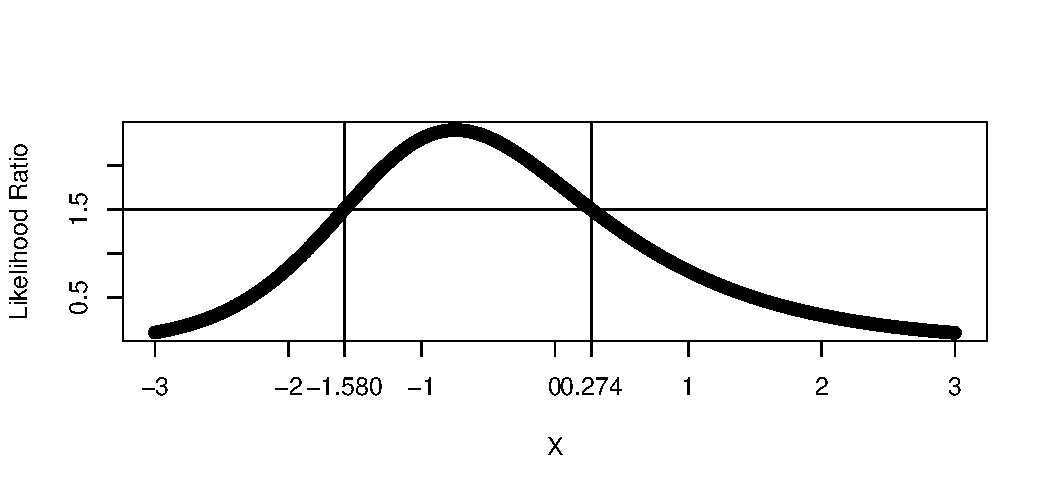
\includegraphics{Homework2-002}
\end{center}
\end{figure} 

The optimal classifier regions are $\ovec{1} = (-1.58,.274)$ and $\ovec{0} = (-\inf,-1.58) \cup (.274,\inf)$
\newpage
\item Performing K-nearest neighbor classification on The Scenario One and Two data from Homework 1 gives the results summarized below.
% latex table generated in R 2.15.1 by xtable 1.7-1 package
% Mon Feb 18 22:14:57 2013
\begin{table}[ht]
\centering
\begin{tabular}{rrrrrrrrrrrrrr}
  \hline
 & 1 & 4 & 7 & 10 & 13 & 16 & 30 & 45 & 60 & 80 & 100 & 150 & 200 \\ 
  \hline
Scen 1 Training Error & 0.0 & 23.5 & 22.5 & 23.0 & 22.0 & 23.5 & 25.0 & 23.0 & 24.0 & 23.0 & 22.0 & 25.5 & 49.0 \\ 
  Scen 1 Testing Error & 30.6 & 28.3 & 25.7 & 27.0 & 26.7 & 25.7 & 26.0 & 24.9 & 25.1 & 24.1 & 24.5 & 23.6 & 52.3 \\ 
  Scen 2 Training Error & 0.0 & 13.0 & 13.0 & 16.0 & 14.5 & 14.0 & 14.5 & 14.0 & 14.0 & 14.5 & 13.5 & 14.5 & 47.5 \\ 
  Scen 2 Testing Error & 16.1 & 13.9 & 13.8 & 12.3 & 12.1 & 12.3 & 12.8 & 13.6 & 13.8 & 13.3 & 13.3 & 13.0 & 51.8 \\ 
   \hline
\end{tabular}
\caption{Training and testing errors for k-nearest neighbor fitting with k-values ranging from 1 to 200}
\end{table}  \begin{enumerate}
    \item Plotting the test and training errors for scenario 1 gives.
   \begin{figure}[h]
\begin{center}
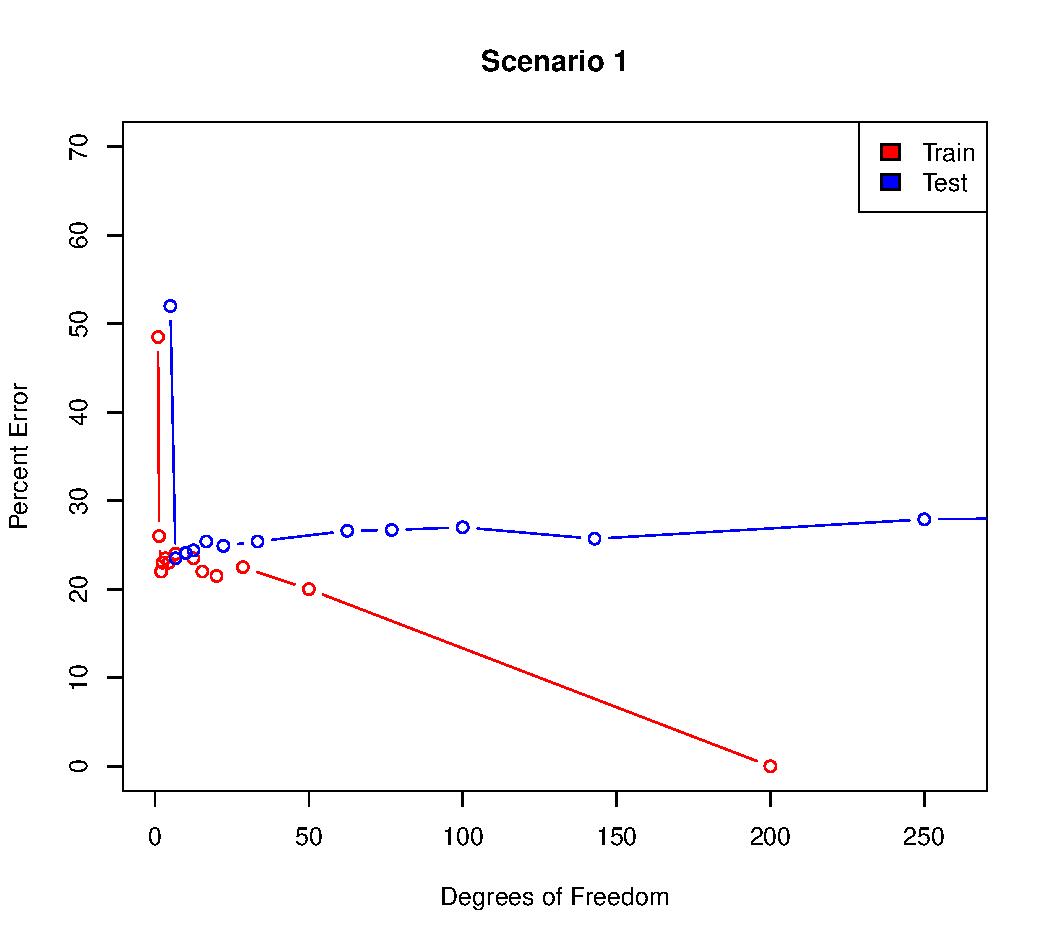
\includegraphics{Homework2-004}
\end{center}
\end{figure} \newpage
  \item Plotting the test and training errors for scenario 2 gives.
   \begin{figure}[h]
\begin{center}
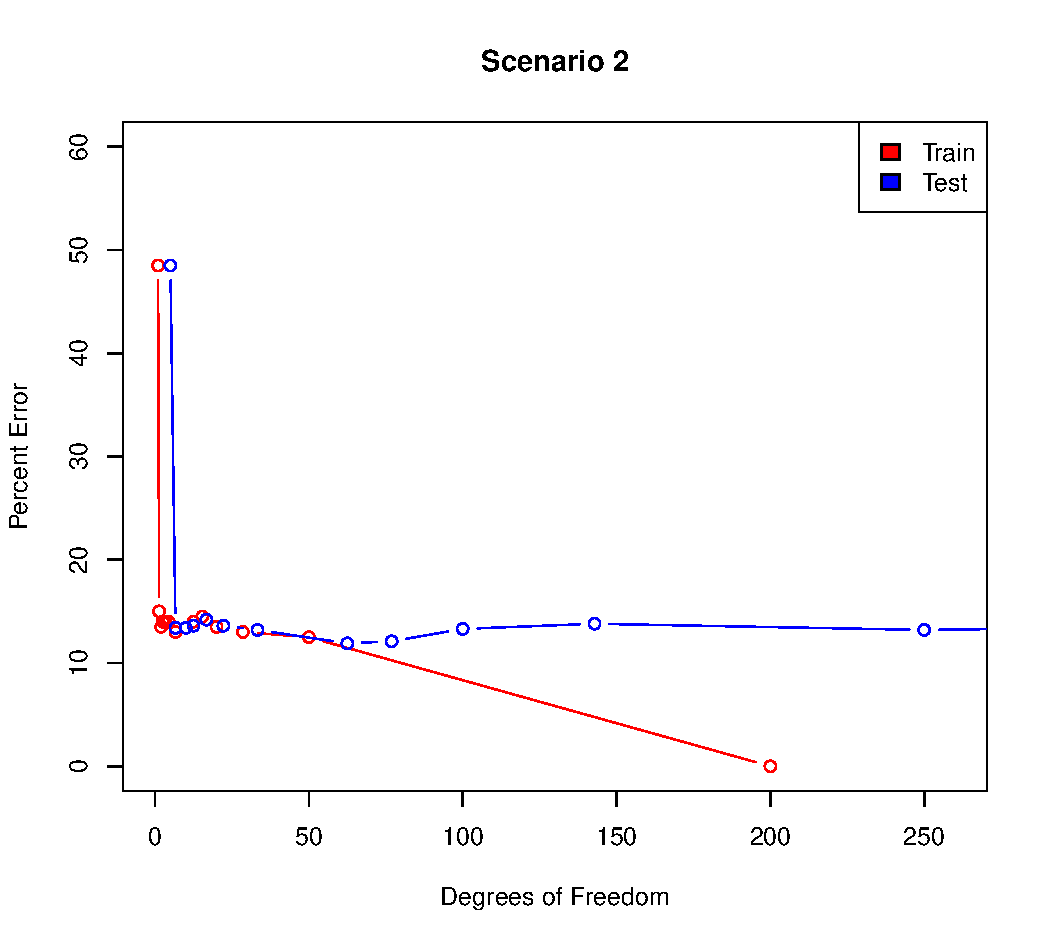
\includegraphics{Homework2-005}
\end{center}
\end{figure}
    \item For both scenarios, k=200 creates very high testing and training error. This makes intuitive sense because for the training sets k=200 means every point in the data set is being compared so there is no clustering at all and there is only one degree of freedom. The error rates get much better as soon as k drops below the number of data points. The error in the training set goes to zero as expected in the case where k=1. The training error tends to decrease in scenario 1 as k increases up to 150, where the best training error is found. In contrast, for scenario 2 the testing error is lowest at k=13. In general we would to choose the value for k that performs best on the test set, so in this case I would choose k=150 for scenario 1 and k=13 for scenario 2.
  \end{enumerate}\newpage
  \item 
    \begin{enumerate}
      \item After running a logistic regression on the data for scenario 1 I find the training error is 26\% and the test error is 23.6\%
      \item After running a logistic regression on the data for scenario 2 I find the training error is 15\% and the testing error is 14.2\%
      \item For both scenarios the classifier performs better on the test data than the training data. As in the k-nearest neighbors classifier, it works substantially better on scenario 2 than on scenario 1.
    \end{enumerate}
  \item
    \begin{enumerate}
      \item After running the LDA classifier on the data for scenario 1 I find the training error is 25\% and the test error is 23.2\%
      \item After running the LDA classifier on the data for scenario 2 I find the training error is 14\% and the testing error is 14.1\%
      \item The LDA classifier performs better in the test data than training data for scenario 1, but for scenario 2 the training error is slightly lower. As in the k-nearest neighbors classifier, it works substantially better on scenario 2 than on scenario 1.
    \end{enumerate}
\end{enumerate}















\end{document}







